% Fluxograma do algoritmo guloso randomizado reativo
\usetikzlibrary{arrows.meta, shapes.geometric}
\tikzset{%
    >={Latex[width=2mm,length=2mm]},
    bloco/.style    = {rectangle, rounded corners, draw=black, fill=blue!10,
                       minimum width=4.5cm, minimum height=0.9cm,
                       text centered, font=\small},
    decisao/.style  = {diamond, draw=black, fill=orange!20, aspect=2.5,
                       text centered, font=\small},
    termino/.style  = {rectangle, rounded corners, draw=black, fill=gray!20,
                       minimum width=4.5cm, minimum height=0.9cm,
                       text centered, font=\small},
}
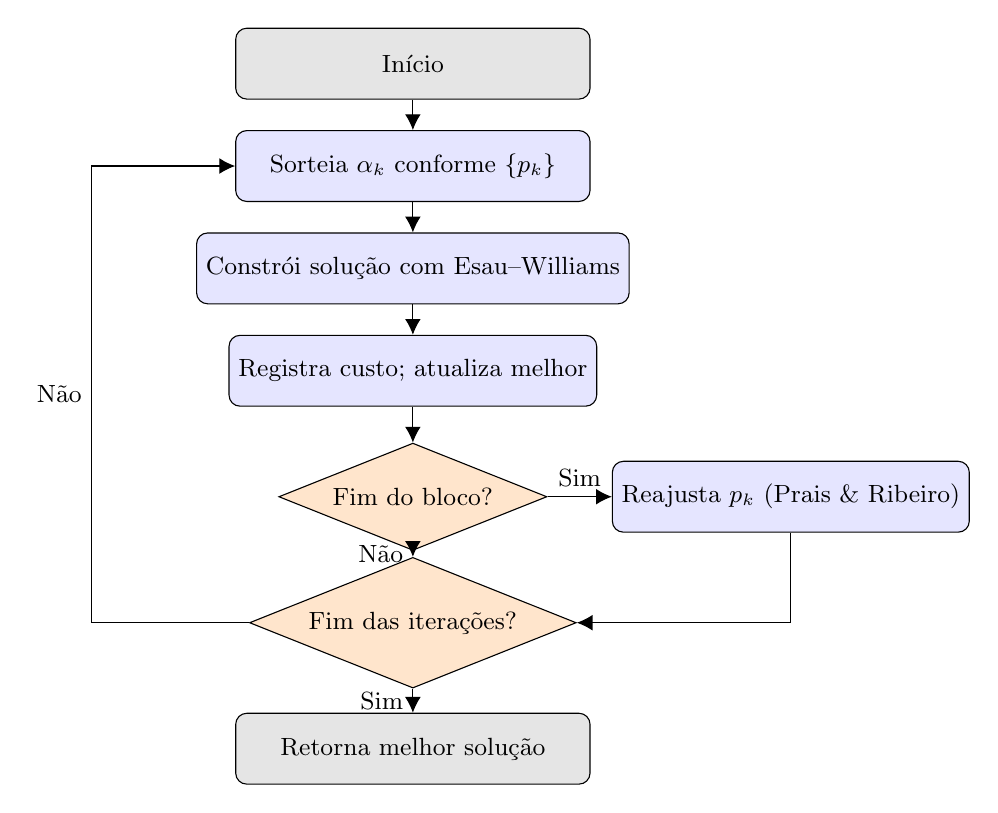
\begin{tikzpicture}[node distance=1.3cm, every node/.style={align=center}]
    \node (ini)   [termino]  {Início};
    \node (prob)  [bloco, below of=ini]   {Sorteia $\alpha_k$ conforme $\{p_k\}$};
    \node (cons)  [bloco, below of=prob]  {Constrói solução com Esau--Williams};
    \node (upd)   [bloco, below of=cons]  {Registra custo; atualiza melhor};
    \node (bloco) [decisao, below of=upd, yshift=-0.3cm] {Fim do bloco?};
    \node (prob2) [bloco, right of=bloco, xshift=3.5cm] {Reajusta $p_k$ (Prais \& Ribeiro)};
    \node (iter)  [decisao, below of=bloco, yshift=-0.3cm] {Fim das iterações?};
    \node (fim)   [termino, below of=iter, yshift=-0.3cm] {Retorna melhor solução};

    \draw[->] (ini)   -- (prob);
    \draw[->] (prob)  -- (cons);
    \draw[->] (cons)  -- (upd);
    \draw[->] (upd)   -- (bloco);
    \draw[->] (bloco) -- node[above, font=\small] {Sim} (prob2);
    \draw[->] (prob2) |- (iter);
    \draw[->] (bloco) -- node[left,  font=\small] {Não} (iter);
    \draw[->] (iter)  -- node[left,  font=\small] {Sim} (fim);
    \draw[->] (iter.west) -- ++(-2,0) |- node[left, font=\small, pos=0.25] {Não} (prob.west);
\end{tikzpicture}
